\RequirePackage{luatex85,shellesc}
\documentclass[crop,tikz]{standalone}
\usepackage{pgfplots}
\usepackage{tikz}
\usepackage[sfdefault]{FiraSans}

\usetikzlibrary{positioning, calc, shapes, arrows, arrows.meta}

\begin{document}

\Large

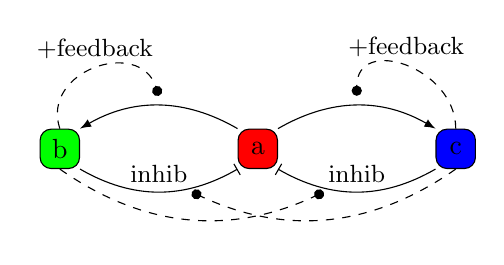
\begin{tikzpicture}[scale=1, every node/.style={}
    , every edge/.style={very thick}
    ]

    \node[minimum size=0.5cm, rounded corners, draw, fill=green] (b) {b};
    \node[minimum size=0.5cm, rounded corners, draw, fill=red, right=2cm of b] (a) {a};
    \node[minimum size=0.5cm, rounded corners, draw, fill=blue, right=2cm of a] (c) {c};
    
    \draw[-|] (b.south east) to[bend right] 
        node[above, midway] (inhb) {\small inhib} (a.south west);

    \draw[latex-] (b.north east) to[bend left] 
        node[above, midway] (prodb) {} (a.north west);

    \draw[|-] (a.south east) to[bend right] 
        node[above, midway] (inhc) {\small inhib} (c.south west);

    \draw[-latex] (a.north east) to[bend left] 
        node[above, midway] (prodc) {} (c.north west);

    % Now c and b catalyze their production.
    \draw[-Circle, dashed] (b.south) to[bend right] 
        node[above, midway] {} (inhc);

    \draw[-Circle, dashed] (b.north) to[bend left,out=90,in=90,looseness=1.5] 
        node[above, midway] {\small +feedback} (prodb.center);


    \draw[-Circle, dashed] (c.north) to[out=90,in=90,looseness=1.5] 
        node[above, midway] {\small +feedback} (prodc.center);

    \draw[-Circle, dashed] (c.south) to[bend left] 
        node[above, midway] {} (inhb);




\end{tikzpicture}	

\end{document}

